\section{Login and Registration}

\begin{figure}[htb]
	\centering
	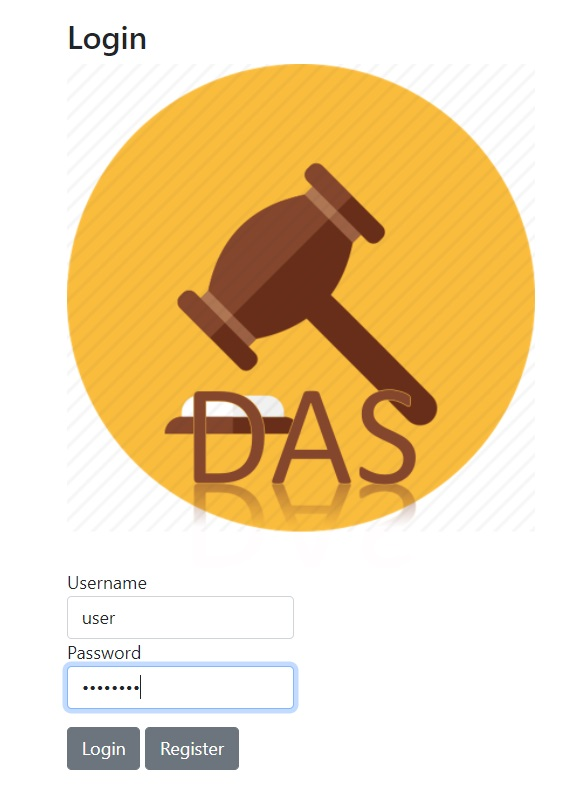
\includegraphics[width=\textwidth]{img/login.jpg}
	\caption{Login interface}\label{fig:login}
\end{figure}

When the application starts it opens the main page (\figref{fig:login}), on
which an old user can insert username and password to login, clicking on the
button ``Login''.

Otherwise, if the user is a new one, he must do the registration procedure.

\subsection{Registration}

If you are a new user, click on ``Register'' on the main page to open the
registration form (\figref{fig:registration}).

Then, insert your username and your password. Insert another time your password
to confirm. If you went in the registration page wrongly, click on ``Login'' to
return to the login page.

\begin{figure}[htb]
	\centering
	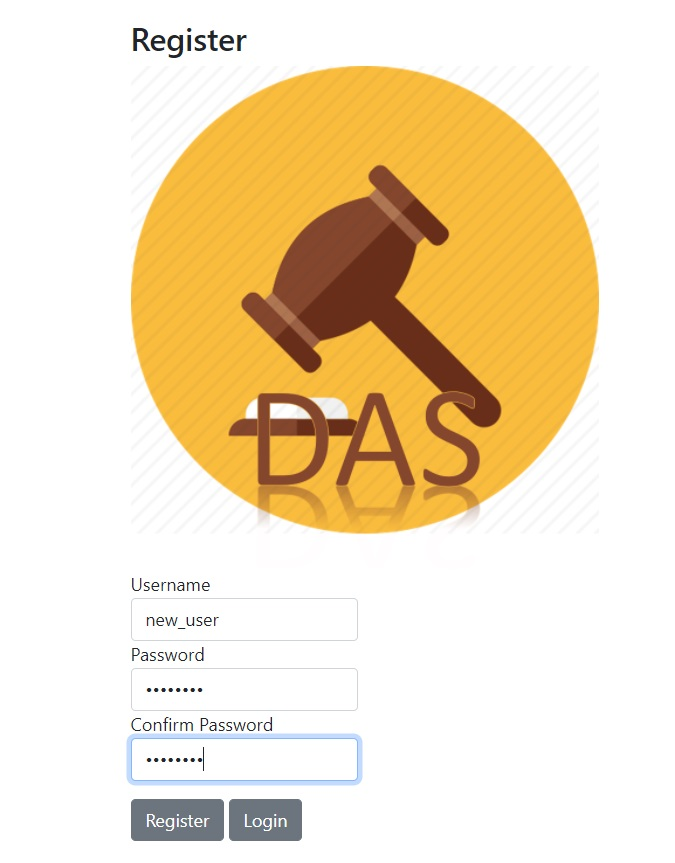
\includegraphics[width=\textwidth]{img/registration.jpg}
	\caption{Registration of a user}\label{fig:registration}
\end{figure}

When you filled out the form, click on ``Register''. Now if you don’t receive
error messages your account will be create. So, login to see all the application
features.
